% Created by tikzDevice version 0.6.1 on 2016-06-13 09:53:13
% !TEX encoding = UTF-8 Unicode
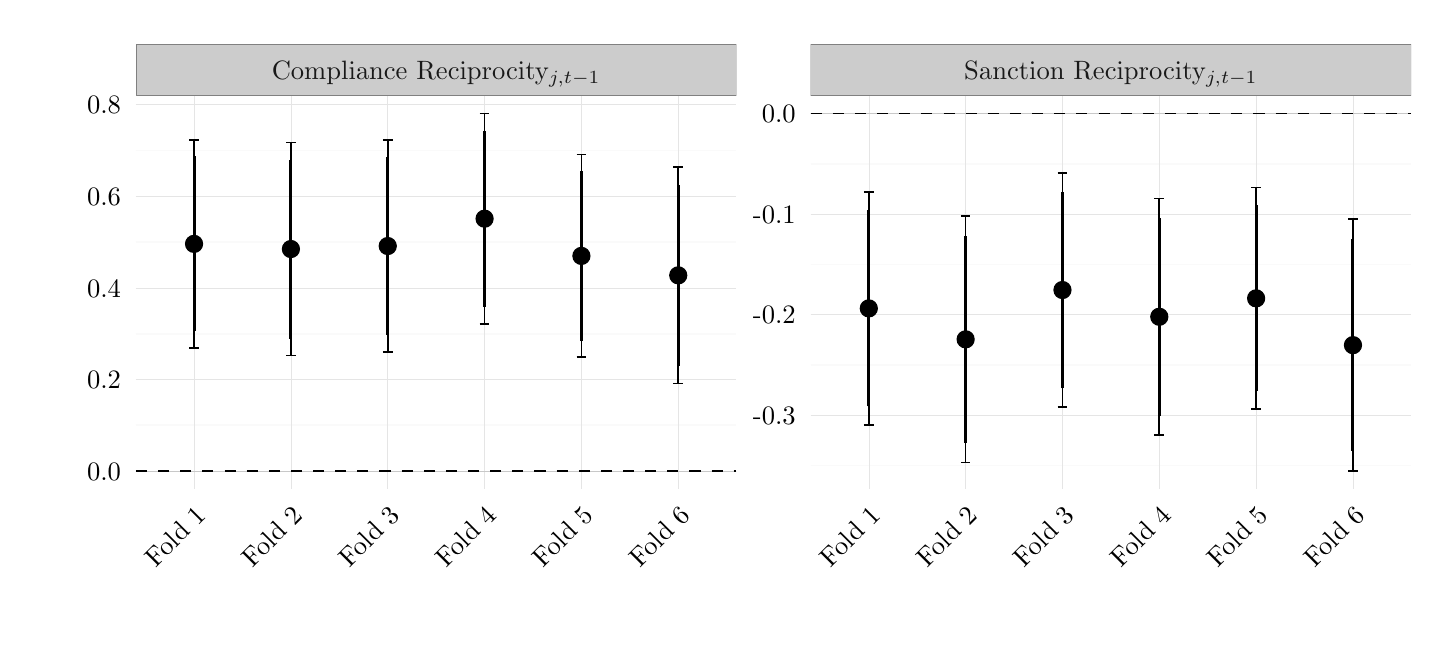
\begin{tikzpicture}[x=1pt,y=1pt]
\definecolor[named]{drawColor}{rgb}{0.00,0.00,0.00}
\definecolor[named]{fillColor}{rgb}{1.00,1.00,1.00}
\fill[color=fillColor,] (0,0) rectangle (505.89,216.81);
\begin{scope}
\path[clip] (  0.00,  0.00) rectangle (505.89,216.81);
\end{scope}
\begin{scope}
\path[clip] (  0.00,  0.00) rectangle (505.89,216.81);
\end{scope}
\begin{scope}
\path[clip] (  0.00,  0.00) rectangle (505.89,216.81);
\end{scope}
\begin{scope}
\path[clip] (  0.00,  0.00) rectangle (505.89,216.81);
\end{scope}
\begin{scope}
\path[clip] (  0.00,  0.00) rectangle (505.89,216.81);
\end{scope}
\begin{scope}
\path[clip] (  0.00,  0.00) rectangle (505.89,216.81);
\end{scope}
\begin{scope}
\path[clip] (  0.00,  0.00) rectangle (505.89,216.81);
\end{scope}
\begin{scope}
\path[clip] (  0.00,  0.00) rectangle (505.89,216.81);
\end{scope}
\begin{scope}
\path[clip] (  0.00,  0.00) rectangle (505.89,216.81);
\end{scope}
\begin{scope}
\path[clip] (  0.00,  0.00) rectangle (505.89,216.81);
\end{scope}
\begin{scope}
\path[clip] (  0.00,  0.00) rectangle (505.89,216.81);
\end{scope}
\begin{scope}
\path[clip] (  0.00,  0.00) rectangle (505.89,216.81);
\end{scope}
\begin{scope}
\path[clip] (  0.00,  0.00) rectangle (505.89,216.81);
\end{scope}
\begin{scope}
\path[clip] (  0.00,  0.00) rectangle (505.89,216.81);
\end{scope}
\begin{scope}
\path[clip] (  0.00,  0.00) rectangle (505.89,216.81);
\definecolor[named]{drawColor}{rgb}{1.00,1.00,1.00}
\definecolor[named]{fillColor}{rgb}{1.00,1.00,1.00}

\draw[color=drawColor,line width= 0.6pt,line cap=round,line join=round,fill=fillColor,] (  0.00,  0.00) rectangle (505.89,216.81);
\end{scope}
\begin{scope}
\path[clip] (  0.00,  0.00) rectangle (505.89,216.81);
\end{scope}
\begin{scope}
\path[clip] ( 39.13, 50.11) rectangle (256.08,192.20);
\definecolor[named]{fillColor}{rgb}{1.00,1.00,1.00}

\draw[fill=fillColor,draw opacity=0.00,] ( 39.13, 50.11) rectangle (256.08,192.20);
\definecolor[named]{drawColor}{rgb}{0.98,0.98,0.98}

\draw[color=drawColor,line width= 0.6pt,line join=round,fill opacity=0.00,] ( 39.13, 73.12) --
	(256.08, 73.12);

\draw[color=drawColor,line width= 0.6pt,line join=round,fill opacity=0.00,] ( 39.13,106.22) --
	(256.08,106.22);

\draw[color=drawColor,line width= 0.6pt,line join=round,fill opacity=0.00,] ( 39.13,139.32) --
	(256.08,139.32);

\draw[color=drawColor,line width= 0.6pt,line join=round,fill opacity=0.00,] ( 39.13,172.42) --
	(256.08,172.42);
\definecolor[named]{drawColor}{rgb}{0.90,0.90,0.90}

\draw[color=drawColor,line width= 0.2pt,line join=round,fill opacity=0.00,] ( 39.13, 56.57) --
	(256.08, 56.57);

\draw[color=drawColor,line width= 0.2pt,line join=round,fill opacity=0.00,] ( 39.13, 89.67) --
	(256.08, 89.67);

\draw[color=drawColor,line width= 0.2pt,line join=round,fill opacity=0.00,] ( 39.13,122.77) --
	(256.08,122.77);

\draw[color=drawColor,line width= 0.2pt,line join=round,fill opacity=0.00,] ( 39.13,155.87) --
	(256.08,155.87);

\draw[color=drawColor,line width= 0.2pt,line join=round,fill opacity=0.00,] ( 39.13,188.97) --
	(256.08,188.97);

\draw[color=drawColor,line width= 0.2pt,line join=round,fill opacity=0.00,] ( 60.12, 50.11) --
	( 60.12,192.20);

\draw[color=drawColor,line width= 0.2pt,line join=round,fill opacity=0.00,] ( 95.12, 50.11) --
	( 95.12,192.20);

\draw[color=drawColor,line width= 0.2pt,line join=round,fill opacity=0.00,] (130.11, 50.11) --
	(130.11,192.20);

\draw[color=drawColor,line width= 0.2pt,line join=round,fill opacity=0.00,] (165.10, 50.11) --
	(165.10,192.20);

\draw[color=drawColor,line width= 0.2pt,line join=round,fill opacity=0.00,] (200.09, 50.11) --
	(200.09,192.20);

\draw[color=drawColor,line width= 0.2pt,line join=round,fill opacity=0.00,] (235.08, 50.11) --
	(235.08,192.20);
\definecolor[named]{drawColor}{rgb}{0.00,0.00,0.00}
\definecolor[named]{fillColor}{rgb}{0.00,0.00,0.00}

\draw[color=drawColor,line width= 0.3pt,line join=round,fill=fillColor,fill opacity=0.30,draw opacity=0.30,] ( 60.12,101.06) -- ( 60.12,176.31);

\draw[color=drawColor,line width= 0.3pt,line join=round,fill=fillColor,fill opacity=0.30,draw opacity=0.30,] ( 95.12, 98.29) -- ( 95.12,175.35);

\draw[color=drawColor,line width= 0.3pt,line join=round,fill=fillColor,fill opacity=0.30,draw opacity=0.30,] (130.11, 99.71) -- (130.11,176.12);

\draw[color=drawColor,line width= 0.3pt,line join=round,fill=fillColor,fill opacity=0.30,draw opacity=0.30,] (165.10,109.82) -- (165.10,185.74);

\draw[color=drawColor,line width= 0.3pt,line join=round,fill=fillColor,fill opacity=0.30,draw opacity=0.30,] (200.09, 97.69) -- (200.09,170.97);

\draw[color=drawColor,line width= 0.3pt,line join=round,fill=fillColor,fill opacity=0.30,draw opacity=0.30,] (235.08, 88.23) -- (235.08,166.38);
\definecolor[named]{drawColor}{rgb}{0.00,0.00,0.00}
\definecolor[named]{fillColor}{rgb}{0.00,0.00,0.00}

\draw[color=drawColor,line width= 1.1pt,line join=round,fill=fillColor,] ( 60.12,107.10) -- ( 60.12,170.26);

\draw[color=drawColor,line width= 1.1pt,line join=round,fill=fillColor,] ( 95.12,104.48) -- ( 95.12,169.16);

\draw[color=drawColor,line width= 1.1pt,line join=round,fill=fillColor,] (130.11,105.85) -- (130.11,169.98);

\draw[color=drawColor,line width= 1.1pt,line join=round,fill=fillColor,] (165.10,115.92) -- (165.10,179.64);

\draw[color=drawColor,line width= 1.1pt,line join=round,fill=fillColor,] (200.09,103.58) -- (200.09,165.08);

\draw[color=drawColor,line width= 1.1pt,line join=round,fill=fillColor,] (235.08, 94.51) -- (235.08,160.10);

\draw[color=drawColor,line width= 0.6pt,dash pattern=on 4pt off 4pt ,line join=round,fill=fillColor,] ( 39.13, 56.57) -- (256.08, 56.57);

\draw[color=drawColor,line width= 0.4pt,line cap=round,line join=round,fill=fillColor,] ( 60.12,138.68) circle (  3.09);

\draw[color=drawColor,line width= 0.4pt,line cap=round,line join=round,fill=fillColor,] ( 95.12,136.82) circle (  3.09);

\draw[color=drawColor,line width= 0.4pt,line cap=round,line join=round,fill=fillColor,] (130.11,137.91) circle (  3.09);

\draw[color=drawColor,line width= 0.4pt,line cap=round,line join=round,fill=fillColor,] (165.10,147.78) circle (  3.09);

\draw[color=drawColor,line width= 0.4pt,line cap=round,line join=round,fill=fillColor,] (200.09,134.33) circle (  3.09);

\draw[color=drawColor,line width= 0.4pt,line cap=round,line join=round,fill=fillColor,] (235.08,127.31) circle (  3.09);

\draw[color=drawColor,line width= 0.6pt,line join=round,] ( 58.37,176.31) --
	( 61.87,176.31);

\draw[color=drawColor,line width= 0.6pt,line join=round,] ( 60.12,176.31) --
	( 60.12,101.06);

\draw[color=drawColor,line width= 0.6pt,line join=round,] ( 58.37,101.06) --
	( 61.87,101.06);

\draw[color=drawColor,line width= 0.6pt,line join=round,] ( 93.37,175.35) --
	( 96.86,175.35);

\draw[color=drawColor,line width= 0.6pt,line join=round,] ( 95.12,175.35) --
	( 95.12, 98.29);

\draw[color=drawColor,line width= 0.6pt,line join=round,] ( 93.37, 98.29) --
	( 96.86, 98.29);

\draw[color=drawColor,line width= 0.6pt,line join=round,] (128.36,176.12) --
	(131.86,176.12);

\draw[color=drawColor,line width= 0.6pt,line join=round,] (130.11,176.12) --
	(130.11, 99.71);

\draw[color=drawColor,line width= 0.6pt,line join=round,] (128.36, 99.71) --
	(131.86, 99.71);

\draw[color=drawColor,line width= 0.6pt,line join=round,] (163.35,185.74) --
	(166.85,185.74);

\draw[color=drawColor,line width= 0.6pt,line join=round,] (165.10,185.74) --
	(165.10,109.82);

\draw[color=drawColor,line width= 0.6pt,line join=round,] (163.35,109.82) --
	(166.85,109.82);

\draw[color=drawColor,line width= 0.6pt,line join=round,] (198.34,170.97) --
	(201.84,170.97);

\draw[color=drawColor,line width= 0.6pt,line join=round,] (200.09,170.97) --
	(200.09, 97.69);

\draw[color=drawColor,line width= 0.6pt,line join=round,] (198.34, 97.69) --
	(201.84, 97.69);

\draw[color=drawColor,line width= 0.6pt,line join=round,] (233.33,166.38) --
	(236.83,166.38);

\draw[color=drawColor,line width= 0.6pt,line join=round,] (235.08,166.38) --
	(235.08, 88.23);

\draw[color=drawColor,line width= 0.6pt,line join=round,] (233.33, 88.23) --
	(236.83, 88.23);
\end{scope}
\begin{scope}
\path[clip] (  0.00,  0.00) rectangle (505.89,216.81);
\end{scope}
\begin{scope}
\path[clip] (282.94, 50.11) rectangle (499.89,192.20);
\definecolor[named]{fillColor}{rgb}{1.00,1.00,1.00}

\draw[fill=fillColor,draw opacity=0.00,] (282.94, 50.11) rectangle (499.89,192.20);
\definecolor[named]{drawColor}{rgb}{0.98,0.98,0.98}

\draw[color=drawColor,line width= 0.6pt,line join=round,fill opacity=0.00,] (282.94, 58.66) --
	(499.89, 58.66);

\draw[color=drawColor,line width= 0.6pt,line join=round,fill opacity=0.00,] (282.94, 94.97) --
	(499.89, 94.97);

\draw[color=drawColor,line width= 0.6pt,line join=round,fill opacity=0.00,] (282.94,131.28) --
	(499.89,131.28);

\draw[color=drawColor,line width= 0.6pt,line join=round,fill opacity=0.00,] (282.94,167.58) --
	(499.89,167.58);
\definecolor[named]{drawColor}{rgb}{0.90,0.90,0.90}

\draw[color=drawColor,line width= 0.2pt,line join=round,fill opacity=0.00,] (282.94, 76.81) --
	(499.89, 76.81);

\draw[color=drawColor,line width= 0.2pt,line join=round,fill opacity=0.00,] (282.94,113.12) --
	(499.89,113.12);

\draw[color=drawColor,line width= 0.2pt,line join=round,fill opacity=0.00,] (282.94,149.43) --
	(499.89,149.43);

\draw[color=drawColor,line width= 0.2pt,line join=round,fill opacity=0.00,] (282.94,185.74) --
	(499.89,185.74);

\draw[color=drawColor,line width= 0.2pt,line join=round,fill opacity=0.00,] (303.94, 50.11) --
	(303.94,192.20);

\draw[color=drawColor,line width= 0.2pt,line join=round,fill opacity=0.00,] (338.93, 50.11) --
	(338.93,192.20);

\draw[color=drawColor,line width= 0.2pt,line join=round,fill opacity=0.00,] (373.92, 50.11) --
	(373.92,192.20);

\draw[color=drawColor,line width= 0.2pt,line join=round,fill opacity=0.00,] (408.91, 50.11) --
	(408.91,192.20);

\draw[color=drawColor,line width= 0.2pt,line join=round,fill opacity=0.00,] (443.90, 50.11) --
	(443.90,192.20);

\draw[color=drawColor,line width= 0.2pt,line join=round,fill opacity=0.00,] (478.89, 50.11) --
	(478.89,192.20);
\definecolor[named]{drawColor}{rgb}{0.00,0.00,0.00}
\definecolor[named]{fillColor}{rgb}{0.00,0.00,0.00}

\draw[color=drawColor,line width= 0.3pt,line join=round,fill=fillColor,fill opacity=0.30,draw opacity=0.30,] (303.94, 73.22) -- (303.94,157.53);

\draw[color=drawColor,line width= 0.3pt,line join=round,fill=fillColor,fill opacity=0.30,draw opacity=0.30,] (338.93, 59.66) -- (338.93,148.71);

\draw[color=drawColor,line width= 0.3pt,line join=round,fill=fillColor,fill opacity=0.30,draw opacity=0.30,] (373.92, 79.71) -- (373.92,164.32);

\draw[color=drawColor,line width= 0.3pt,line join=round,fill=fillColor,fill opacity=0.30,draw opacity=0.30,] (408.91, 69.61) -- (408.91,155.06);

\draw[color=drawColor,line width= 0.3pt,line join=round,fill=fillColor,fill opacity=0.30,draw opacity=0.30,] (443.90, 78.99) -- (443.90,159.01);

\draw[color=drawColor,line width= 0.3pt,line join=round,fill=fillColor,fill opacity=0.30,draw opacity=0.30,] (478.89, 56.57) -- (478.89,147.61);
\definecolor[named]{drawColor}{rgb}{0.00,0.00,0.00}
\definecolor[named]{fillColor}{rgb}{0.00,0.00,0.00}

\draw[color=drawColor,line width= 1.1pt,line join=round,fill=fillColor,] (303.94, 79.99) -- (303.94,150.75);

\draw[color=drawColor,line width= 1.1pt,line join=round,fill=fillColor,] (338.93, 66.82) -- (338.93,141.55);

\draw[color=drawColor,line width= 1.1pt,line join=round,fill=fillColor,] (373.92, 86.51) -- (373.92,157.51);

\draw[color=drawColor,line width= 1.1pt,line join=round,fill=fillColor,] (408.91, 76.48) -- (408.91,148.19);

\draw[color=drawColor,line width= 1.1pt,line join=round,fill=fillColor,] (443.90, 85.42) -- (443.90,152.58);

\draw[color=drawColor,line width= 1.1pt,line join=round,fill=fillColor,] (478.89, 63.89) -- (478.89,140.29);

\draw[color=drawColor,line width= 0.6pt,dash pattern=on 4pt off 4pt ,line join=round,fill=fillColor,] (282.94,185.74) -- (499.89,185.74);

\draw[color=drawColor,line width= 0.4pt,line cap=round,line join=round,fill=fillColor,] (303.94,115.37) circle (  3.09);

\draw[color=drawColor,line width= 0.4pt,line cap=round,line join=round,fill=fillColor,] (338.93,104.19) circle (  3.09);

\draw[color=drawColor,line width= 0.4pt,line cap=round,line join=round,fill=fillColor,] (373.92,122.01) circle (  3.09);

\draw[color=drawColor,line width= 0.4pt,line cap=round,line join=round,fill=fillColor,] (408.91,112.34) circle (  3.09);

\draw[color=drawColor,line width= 0.4pt,line cap=round,line join=round,fill=fillColor,] (443.90,119.00) circle (  3.09);

\draw[color=drawColor,line width= 0.4pt,line cap=round,line join=round,fill=fillColor,] (478.89,102.09) circle (  3.09);

\draw[color=drawColor,line width= 0.6pt,line join=round,] (302.19,157.53) --
	(305.69,157.53);

\draw[color=drawColor,line width= 0.6pt,line join=round,] (303.94,157.53) --
	(303.94, 73.22);

\draw[color=drawColor,line width= 0.6pt,line join=round,] (302.19, 73.22) --
	(305.69, 73.22);

\draw[color=drawColor,line width= 0.6pt,line join=round,] (337.18,148.71) --
	(340.68,148.71);

\draw[color=drawColor,line width= 0.6pt,line join=round,] (338.93,148.71) --
	(338.93, 59.66);

\draw[color=drawColor,line width= 0.6pt,line join=round,] (337.18, 59.66) --
	(340.68, 59.66);

\draw[color=drawColor,line width= 0.6pt,line join=round,] (372.17,164.32) --
	(375.67,164.32);

\draw[color=drawColor,line width= 0.6pt,line join=round,] (373.92,164.32) --
	(373.92, 79.71);

\draw[color=drawColor,line width= 0.6pt,line join=round,] (372.17, 79.71) --
	(375.67, 79.71);

\draw[color=drawColor,line width= 0.6pt,line join=round,] (407.16,155.06) --
	(410.66,155.06);

\draw[color=drawColor,line width= 0.6pt,line join=round,] (408.91,155.06) --
	(408.91, 69.61);

\draw[color=drawColor,line width= 0.6pt,line join=round,] (407.16, 69.61) --
	(410.66, 69.61);

\draw[color=drawColor,line width= 0.6pt,line join=round,] (442.15,159.01) --
	(445.65,159.01);

\draw[color=drawColor,line width= 0.6pt,line join=round,] (443.90,159.01) --
	(443.90, 78.99);

\draw[color=drawColor,line width= 0.6pt,line join=round,] (442.15, 78.99) --
	(445.65, 78.99);

\draw[color=drawColor,line width= 0.6pt,line join=round,] (477.15,147.61) --
	(480.64,147.61);

\draw[color=drawColor,line width= 0.6pt,line join=round,] (478.89,147.61) --
	(478.89, 56.57);

\draw[color=drawColor,line width= 0.6pt,line join=round,] (477.15, 56.57) --
	(480.64, 56.57);
\end{scope}
\begin{scope}
\path[clip] (  0.00,  0.00) rectangle (505.89,216.81);
\end{scope}
\begin{scope}
\path[clip] (  0.00,  0.00) rectangle (505.89,216.81);
\end{scope}
\begin{scope}
\path[clip] ( 39.13,192.20) rectangle (256.08,210.81);
\definecolor[named]{drawColor}{rgb}{0.50,0.50,0.50}
\definecolor[named]{fillColor}{rgb}{0.80,0.80,0.80}

\draw[color=drawColor,line width= 0.2pt,line cap=round,line join=round,fill=fillColor,] ( 39.13,192.20) rectangle (256.08,210.81);
\definecolor[named]{drawColor}{rgb}{0.10,0.10,0.10}

\node[color=drawColor,anchor=base,inner sep=0pt, outer sep=0pt, scale=  0.96] at (147.60,198.20) {Compliance Reciprocity$_{j,t-1}$%
};
\end{scope}
\begin{scope}
\path[clip] ( 39.13,192.20) rectangle (256.08,210.81);
\end{scope}
\begin{scope}
\path[clip] (  0.00,  0.00) rectangle (505.89,216.81);
\end{scope}
\begin{scope}
\path[clip] (  0.00,  0.00) rectangle (505.89,216.81);
\end{scope}
\begin{scope}
\path[clip] (  0.00,  0.00) rectangle (505.89,216.81);
\end{scope}
\begin{scope}
\path[clip] (282.94,192.20) rectangle (499.89,210.81);
\definecolor[named]{drawColor}{rgb}{0.50,0.50,0.50}
\definecolor[named]{fillColor}{rgb}{0.80,0.80,0.80}

\draw[color=drawColor,line width= 0.2pt,line cap=round,line join=round,fill=fillColor,] (282.94,192.20) rectangle (499.89,210.81);
\definecolor[named]{drawColor}{rgb}{0.10,0.10,0.10}

\node[color=drawColor,anchor=base,inner sep=0pt, outer sep=0pt, scale=  0.96] at (391.42,198.20) {Sanction Reciprocity$_{j,t-1}$%
};
\end{scope}
\begin{scope}
\path[clip] (282.94,192.20) rectangle (499.89,210.81);
\end{scope}
\begin{scope}
\path[clip] (  0.00,  0.00) rectangle (505.89,216.81);
\end{scope}
\begin{scope}
\path[clip] (  0.00,  0.00) rectangle (505.89,216.81);
\end{scope}
\begin{scope}
\path[clip] (  0.00,  0.00) rectangle (505.89,216.81);
\end{scope}
\begin{scope}
\path[clip] (  0.00,  0.00) rectangle (505.89,216.81);
\end{scope}
\begin{scope}
\path[clip] (  0.00,  0.00) rectangle (505.89,216.81);
\end{scope}
\begin{scope}
\path[clip] (  0.00,  0.00) rectangle (505.89,216.81);
\end{scope}
\begin{scope}
\path[clip] (  0.00,  0.00) rectangle (505.89,216.81);
\definecolor[named]{drawColor}{rgb}{0.00,0.00,0.00}

\node[color=drawColor,anchor=base east,inner sep=0pt, outer sep=0pt, scale=  0.96] at ( 33.73, 53.26) {0.0%
};

\node[color=drawColor,anchor=base east,inner sep=0pt, outer sep=0pt, scale=  0.96] at ( 33.73, 86.36) {0.2%
};

\node[color=drawColor,anchor=base east,inner sep=0pt, outer sep=0pt, scale=  0.96] at ( 33.73,119.46) {0.4%
};

\node[color=drawColor,anchor=base east,inner sep=0pt, outer sep=0pt, scale=  0.96] at ( 33.73,152.56) {0.6%
};

\node[color=drawColor,anchor=base east,inner sep=0pt, outer sep=0pt, scale=  0.96] at ( 33.73,185.66) {0.8%
};
\end{scope}
\begin{scope}
\path[clip] (  0.00,  0.00) rectangle (505.89,216.81);
\end{scope}
\begin{scope}
\path[clip] (  0.00,  0.00) rectangle (505.89,216.81);
\end{scope}
\begin{scope}
\path[clip] (  0.00,  0.00) rectangle (505.89,216.81);
\end{scope}
\begin{scope}
\path[clip] (  0.00,  0.00) rectangle (505.89,216.81);
\end{scope}
\begin{scope}
\path[clip] (  0.00,  0.00) rectangle (505.89,216.81);
\end{scope}
\begin{scope}
\path[clip] (  0.00,  0.00) rectangle (505.89,216.81);
\end{scope}
\begin{scope}
\path[clip] (  0.00,  0.00) rectangle (505.89,216.81);
\end{scope}
\begin{scope}
\path[clip] (  0.00,  0.00) rectangle (505.89,216.81);
\end{scope}
\begin{scope}
\path[clip] (  0.00,  0.00) rectangle (505.89,216.81);
\end{scope}
\begin{scope}
\path[clip] (  0.00,  0.00) rectangle (505.89,216.81);
\definecolor[named]{drawColor}{rgb}{0.00,0.00,0.00}

\node[color=drawColor,anchor=base east,inner sep=0pt, outer sep=0pt, scale=  0.96] at (277.54, 73.51) {-0.3%
};

\node[color=drawColor,anchor=base east,inner sep=0pt, outer sep=0pt, scale=  0.96] at (277.54,109.81) {-0.2%
};

\node[color=drawColor,anchor=base east,inner sep=0pt, outer sep=0pt, scale=  0.96] at (277.54,146.12) {-0.1%
};

\node[color=drawColor,anchor=base east,inner sep=0pt, outer sep=0pt, scale=  0.96] at (277.54,182.43) {0.0%
};
\end{scope}
\begin{scope}
\path[clip] (  0.00,  0.00) rectangle (505.89,216.81);
\end{scope}
\begin{scope}
\path[clip] (  0.00,  0.00) rectangle (505.89,216.81);
\end{scope}
\begin{scope}
\path[clip] (  0.00,  0.00) rectangle (505.89,216.81);
\end{scope}
\begin{scope}
\path[clip] (  0.00,  0.00) rectangle (505.89,216.81);
\end{scope}
\begin{scope}
\path[clip] (  0.00,  0.00) rectangle (505.89,216.81);
\end{scope}
\begin{scope}
\path[clip] (  0.00,  0.00) rectangle (505.89,216.81);
\end{scope}
\begin{scope}
\path[clip] (  0.00,  0.00) rectangle (505.89,216.81);
\end{scope}
\begin{scope}
\path[clip] (  0.00,  0.00) rectangle (505.89,216.81);
\end{scope}
\begin{scope}
\path[clip] (  0.00,  0.00) rectangle (505.89,216.81);
\end{scope}
\begin{scope}
\path[clip] (  0.00,  0.00) rectangle (505.89,216.81);
\end{scope}
\begin{scope}
\path[clip] (  0.00,  0.00) rectangle (505.89,216.81);
\end{scope}
\begin{scope}
\path[clip] (  0.00,  0.00) rectangle (505.89,216.81);
\definecolor[named]{drawColor}{rgb}{0.00,0.00,0.00}

\node[rotate= 45.00,color=drawColor,anchor=base east,inner sep=0pt, outer sep=0pt, scale=  0.96] at ( 64.80, 40.03) {Fold 1%
};

\node[rotate= 45.00,color=drawColor,anchor=base east,inner sep=0pt, outer sep=0pt, scale=  0.96] at ( 99.79, 40.03) {Fold 2%
};

\node[rotate= 45.00,color=drawColor,anchor=base east,inner sep=0pt, outer sep=0pt, scale=  0.96] at (134.78, 40.03) {Fold 3%
};

\node[rotate= 45.00,color=drawColor,anchor=base east,inner sep=0pt, outer sep=0pt, scale=  0.96] at (169.77, 40.03) {Fold 4%
};

\node[rotate= 45.00,color=drawColor,anchor=base east,inner sep=0pt, outer sep=0pt, scale=  0.96] at (204.77, 40.03) {Fold 5%
};

\node[rotate= 45.00,color=drawColor,anchor=base east,inner sep=0pt, outer sep=0pt, scale=  0.96] at (239.76, 40.03) {Fold 6%
};
\end{scope}
\begin{scope}
\path[clip] (  0.00,  0.00) rectangle (505.89,216.81);
\end{scope}
\begin{scope}
\path[clip] (  0.00,  0.00) rectangle (505.89,216.81);
\end{scope}
\begin{scope}
\path[clip] (  0.00,  0.00) rectangle (505.89,216.81);
\end{scope}
\begin{scope}
\path[clip] (  0.00,  0.00) rectangle (505.89,216.81);
\end{scope}
\begin{scope}
\path[clip] (  0.00,  0.00) rectangle (505.89,216.81);
\end{scope}
\begin{scope}
\path[clip] (  0.00,  0.00) rectangle (505.89,216.81);
\end{scope}
\begin{scope}
\path[clip] (  0.00,  0.00) rectangle (505.89,216.81);
\end{scope}
\begin{scope}
\path[clip] (  0.00,  0.00) rectangle (505.89,216.81);
\end{scope}
\begin{scope}
\path[clip] (  0.00,  0.00) rectangle (505.89,216.81);
\end{scope}
\begin{scope}
\path[clip] (  0.00,  0.00) rectangle (505.89,216.81);
\definecolor[named]{drawColor}{rgb}{0.00,0.00,0.00}

\node[rotate= 45.00,color=drawColor,anchor=base east,inner sep=0pt, outer sep=0pt, scale=  0.96] at (308.61, 40.03) {Fold 1%
};

\node[rotate= 45.00,color=drawColor,anchor=base east,inner sep=0pt, outer sep=0pt, scale=  0.96] at (343.60, 40.03) {Fold 2%
};

\node[rotate= 45.00,color=drawColor,anchor=base east,inner sep=0pt, outer sep=0pt, scale=  0.96] at (378.59, 40.03) {Fold 3%
};

\node[rotate= 45.00,color=drawColor,anchor=base east,inner sep=0pt, outer sep=0pt, scale=  0.96] at (413.59, 40.03) {Fold 4%
};

\node[rotate= 45.00,color=drawColor,anchor=base east,inner sep=0pt, outer sep=0pt, scale=  0.96] at (448.58, 40.03) {Fold 5%
};

\node[rotate= 45.00,color=drawColor,anchor=base east,inner sep=0pt, outer sep=0pt, scale=  0.96] at (483.57, 40.03) {Fold 6%
};
\end{scope}
\begin{scope}
\path[clip] (  0.00,  0.00) rectangle (505.89,216.81);
\end{scope}
\begin{scope}
\path[clip] (  0.00,  0.00) rectangle (505.89,216.81);
\end{scope}
\begin{scope}
\path[clip] (  0.00,  0.00) rectangle (505.89,216.81);
\end{scope}
\begin{scope}
\path[clip] (  0.00,  0.00) rectangle (505.89,216.81);
\end{scope}
\begin{scope}
\path[clip] (  0.00,  0.00) rectangle (505.89,216.81);
\end{scope}
\begin{scope}
\path[clip] (  0.00,  0.00) rectangle (505.89,216.81);
\end{scope}
\begin{scope}
\path[clip] (  0.00,  0.00) rectangle (505.89,216.81);
\end{scope}
\begin{scope}
\path[clip] (  0.00,  0.00) rectangle (505.89,216.81);
\end{scope}
\begin{scope}
\path[clip] (  0.00,  0.00) rectangle (505.89,216.81);
\end{scope}
\begin{scope}
\path[clip] (  0.00,  0.00) rectangle (505.89,216.81);
\end{scope}
\end{tikzpicture}
